\documentclass{article}
\usepackage{graphicx} % Required for inserting images
\usepackage[margin=3cm]{geometry}
\usepackage{biblatex}
\usepackage{hyperref}
\usepackage{cleveref}
\usepackage{listings}
\usepackage{tabularx}


\hypersetup{
    colorlinks=true,
    linkcolor=blue,
    filecolor=magenta,      
    urlcolor=cyan,
    pdftitle={Overleaf Example},
    pdfpagemode=FullScreen,
    }

\title{NEA \\Route Card and Route Planning tool}
\author{Jonty Beglin}
\date{April 2024}

\newcommand{\Q}{\bigskip\bfseries Q: }
\newcommand{\A}{\par\textbf{A:} \normalfont}

\newcommand{\Adv}{\bigskip\textbf{Advantages: }}
\newcommand{\Dis}{\bigskip\textbf{Disadvantages: }}

\newcommand{\QAnalysis}[4]{
    \noindent \textbf{Question #1: } #2 \\
    \noindent \textbf{Answer(s): } #3
    \begin{itemize}
        \item #4
    \end{itemize}
}

\newcommand{\testtable}[6]{
    \begin{center}
        \textbf{#1}
        \vspace{0.125cm}
        \vspace{0.25cm}
        \begin{tabularx}{\textwidth}{ |X|X|X|X| }
            \hline
            Testing & Objective & Pass/Fail & Notes \\
            \hline
            #2 & #3 & #4 & #5 \\
            \hline
        \end{tabularx}
        \\
        \vspace{0.25cm}
        \url{#6}
    \end{center}
}

\begin{document}

\maketitle

\newpage

\tableofcontents

\newpage


\section{Analysis}

    \subsection{The Problem}

        I would like to create a tool that allows users to plan hiking routes on an interactive UI featuring a map and waypoint capabilities. The tool should then be able to return to the user a route card that the user can use while on their hike to navigate along the path they have created within the program with useful information they may want such as bearings, walking times, distances and place names. An example of what could be displayed in the program can be seen in \cref{fig:example_map_dartmoor}.

        \begin{figure}[ht]
            \centering
            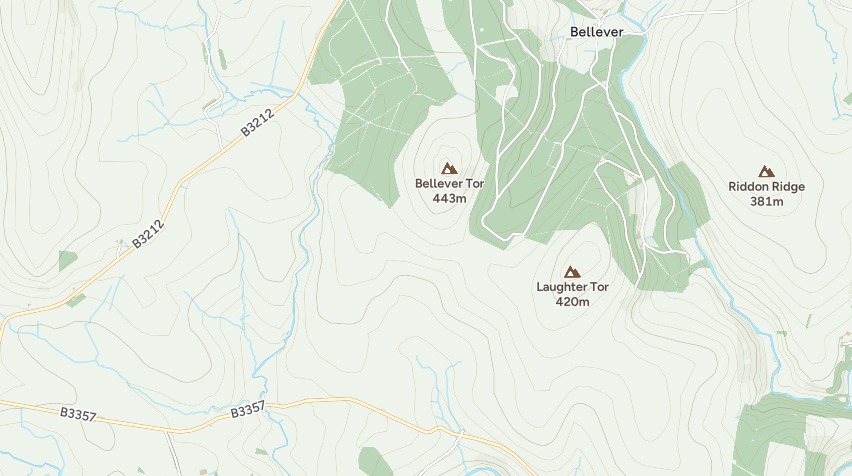
\includegraphics[width=0.75\textwidth]{Photos/Example/OSmapsExampleDartmoor.png}
            \caption{Example of a map which could be displayed within the program}
            \label{fig:example_map_dartmoor}
         \end{figure}

         Currently many people I know use pen and paper with physical maps to measure out distance and do manual calculations to create their route cards. I believe many people would benefit from this as it should be faster, easier and more accurate than traditional methods. I would further like to add options to load and save routes meaning users can edit their previously created routes.
         
         I would like to implement a feature to snap to paths to get more accurate readings of the path distance and time taken to walk a path. However, depending on which APIs are used and what data is available this may not be possible to achieve in some circumstances due to the disparity between the real world and the data online.
         
        \begin{figure}[ht]
            \centering
            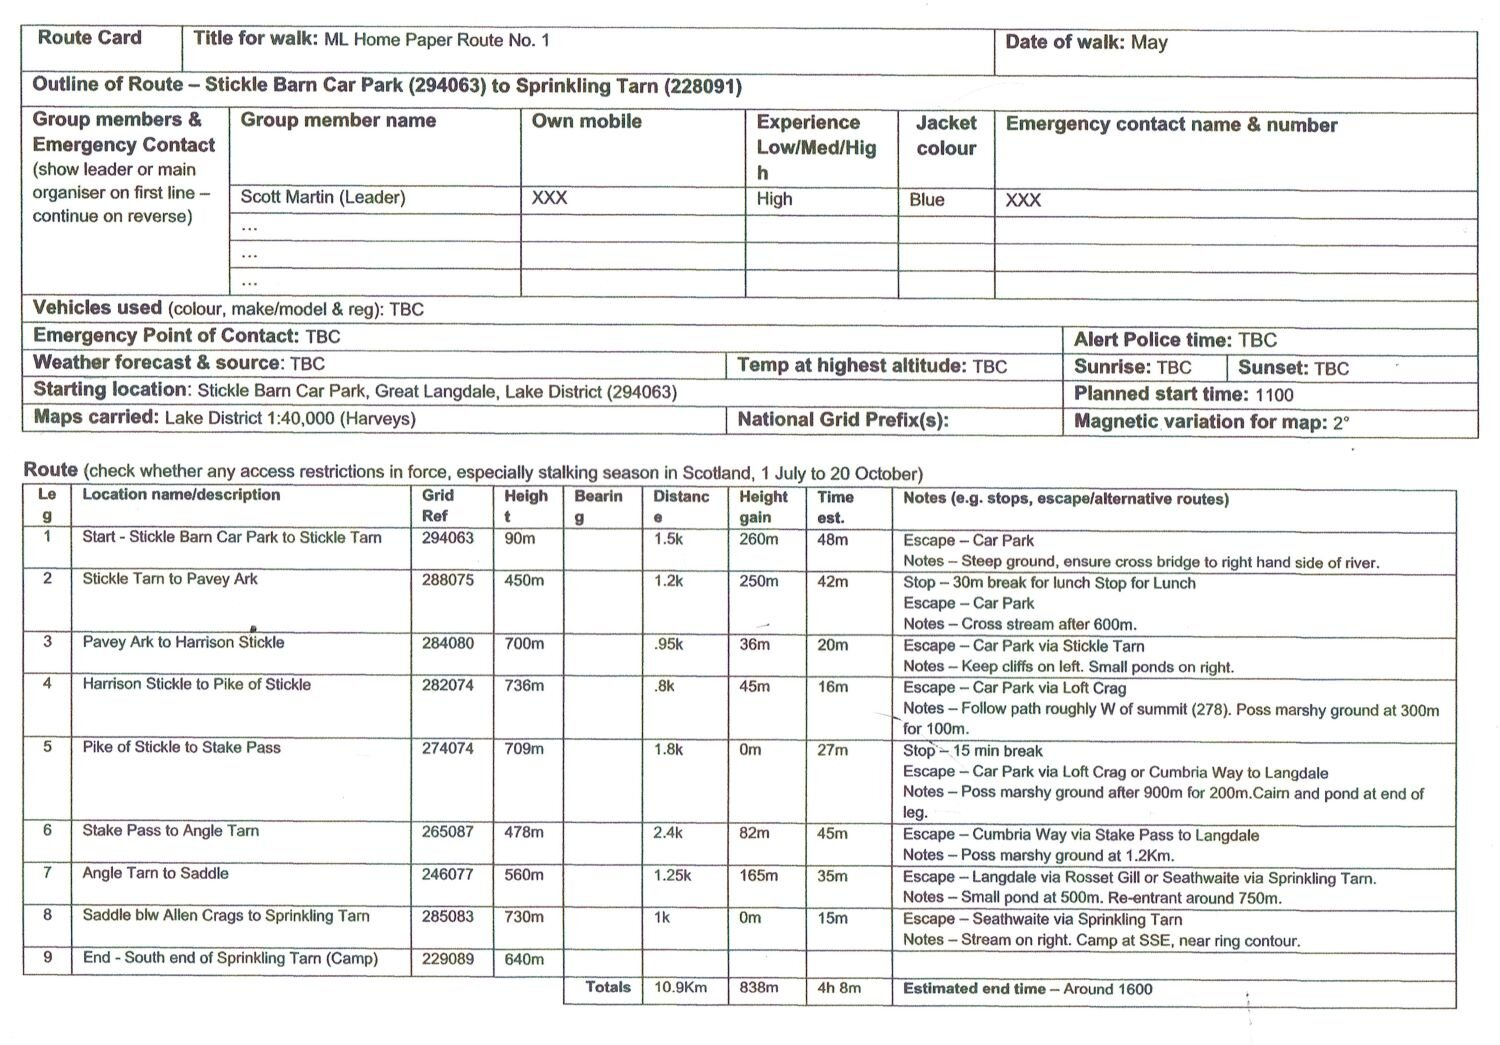
\includegraphics[width=0.75\textwidth]{Photos/Example/RouteCardExample.jpg}
            \caption{Example of a Route Card which could be generated from the program}
            \label{fig:example_route_card}
         \end{figure}
         
         I think there should be options for how the route card will be laid out, potentially allowing the user to directly edit the route card which will be outputted. This may be a sub-program within the main program which enables the user to view and edit the data of the route card. An example route card which the program should aim to output can be seen in \cref{fig:example_route_card}.

    \subsection{Mapping APIs}

        Choosing the most suitable API for gathering map data is paramount to the project's success. The map data needs to be able to be accessed relatively quickly and reliably, the user could potentially interact with an interactive map as seen in Google Maps and draw the route in real-time, however, this may be out of the scope of the project, so instead I could allow the user to use an interactive map to find a snapshot location of their "work area" where then they can draw their route on top of which will have an inbuilt scale automatically scaled to the same scale as when they were using the interactive map. The user's waypoint locations could be saved to allow for the later creation of a route card or as previously mentioned create a route which can be edited or expanded upon later. Optimally the mapping API should allow me to feed in some latitude and longitude and it feed back some mapping data in the form of a photo or other source which can then be overlaid onto the screen and I could use some module such as pygame or tkinter in python to move based on the user's actions.

        \subsubsection{Google Maps}

            The Google Maps API seems to be the most popular mapping API used by businesses and for some personal use. Upon the creation of a Google developer account and attempting to generate an API key I was prompted to input card details for future payment which is out of the question for this project. Furthermore, I believe the Google Maps API is more suitable for businesses displaying their locations in a browser with Google Maps meaning users can more easily see where the business is located. I tried for a while to attempt to use the Google Maps map tiles API to get terrain tiles and satellite tiles both of which did not work as I could not successfully generate a session token. Here is the code I was using to attempt to generate a session token, replacing API\_KEY with my API key generated by Google.

            \definecolor{codegreen}{rgb}{0,0.6,0}
            \definecolor{codegray}{rgb}{0.5,0.5,0.5}
            \definecolor{codepurple}{rgb}{0.58,0,0.82}
            \definecolor{backcolour}{rgb}{0.95,0.95,0.92}
        
            \lstdefinestyle{mystyle}{
                backgroundcolor=\color{backcolour},   
                commentstyle=\color{codegreen},
                keywordstyle=\color{magenta},
                numberstyle=\tiny\color{codegray},
                stringstyle=\color{codepurple},
                basicstyle=\ttfamily\footnotesize,
                breakatwhitespace=false,         
                breaklines=true,                 
                captionpos=b,                    
                keepspaces=true,                 
                numbers=left,                    
                numbersep=5pt,                  
                showspaces=false,                
                showstringspaces=false,
                showtabs=false,                  
                tabsize=2
            }
        
            \lstset{style=mystyle}
            
            \lstinputlisting[language=Python]{googlemaps.py}

        \subsubsection{here.com}

            

        \subsubsection{Open Layers}



        \subsubsection{TomTom}



        \subsubsection{MapBox}

            

    \subsection{User's Needs}

        \subsubsection{Questionnaire}

            My first method of analysing the user's need is through the use of a questionnaire sent out to the members of a local scout group to receive feedback on how they would want a program like this to functions and what features are the most important to the user. I also asked for any additional feedback which they could not provide through the previous fields. \\
            
            \QAnalysis{1}{How likely would you be to use a computer program to plan your route?}{Very likely, Somewhat likely, neither likely nor unlikely, Somewhat unlikely, Very unlikely}{Asking this question allows me to take into account how much a particular response should affect the way I plan my project. If a potential user is very unlikely to use a computer program to plan their route, I should not focus on tailoring the program to them.}

            \QAnalysis{2}{Which Features would you say are most important to you within the mapping tool?}{Accurate map information with paths on, Easy to use, Being able to move and edit points on the route, Route automatically going along a path, Saving routes}{This question allowed the user to order which features are the most important to them and thus allow me to build an ordered list of priority features which the end user would like to see the most.}

            \QAnalysis{3}{What features about the route card creator are most important to you?}{Automatically fills timings, Being able to edit the route card after creation, Automatically calculates elevation, Automatically calculates bearings, Automatically filled in emergency information}{Similar to the previous question, this allowed the user to order what features are the most important to them within the program but specifically within the route card editor/creator part of the program which highlights the important parts of the route card creator.}

            \QAnalysis{4}{How would you like the route card to be output to you so you can edit it if needed?}{Excel Spreadsheet, PDF, Within the program, Other: specify}{This gives me information about how the users may want the program to output the final route card to them. Creating a route card editor within the program may be hard and potentially less user-friendly, pdf would necessitate research into creating a pdf with adequate formatting.}

            \QAnalysis{5}{What information about each leg do you want?}{From (e.g. From Brentor), To (e.g. To Pewtor), From and To (e.g. From Brentor to Pewtor)}{This question truly dials into how the program should output route cards and what information should be given on on them and what would be most useful the end users.}

            \QAnalysis{6}{If you could have a login to the tool what features would you use (multiple choice)?}{Saving Routes, Saving Safety information (escape notes), Emergency contacts automatically filled in, Saving your typical walking speed, Sharing routes with others}{This was a multiple choice question which allowed users to select multiple of the proposed features allowing me to gauge which are the most important to the most users.}

            \QAnalysis{7}{How do you make your route cards (e.g. paper or online tools)?}{Text Box}{This question is to give me an insight into alternatives allowing me to research them and what their advantages and disadvantages may be so that I can take the pros and cons of each of them and attempt to make an overall superior program.}

            \QAnalysis{8}{Any other comments:}{Text Box}{This allows the respondent to add any additional information or opinions which were not captured by the previous questions.}
    
\newpage

\section{Documented Design}

    

\newpage
    
\section{Technical Solution}

    

\newpage

\section{Testing}

    

\newpage

\section{Evaluation}

    
    
\end{document}
